\documentclass[]{elsarticle} %review=doublespace preprint=single 5p=2 column
%%% Begin My package additions %%%%%%%%%%%%%%%%%%%

\usepackage[hyphens]{url}


\usepackage{lineno} % add
  \linenumbers % turns line numbering on

\usepackage{graphicx}
%%%%%%%%%%%%%%%% end my additions to header

\usepackage[T1]{fontenc}
\usepackage{lmodern}
\usepackage{amssymb,amsmath}
\usepackage{ifxetex,ifluatex}
\usepackage{fixltx2e} % provides \textsubscript
% use upquote if available, for straight quotes in verbatim environments
\IfFileExists{upquote.sty}{\usepackage{upquote}}{}
\ifnum 0\ifxetex 1\fi\ifluatex 1\fi=0 % if pdftex
  \usepackage[utf8]{inputenc}
\else % if luatex or xelatex
  \usepackage{fontspec}
  \ifxetex
    \usepackage{xltxtra,xunicode}
  \fi
  \defaultfontfeatures{Mapping=tex-text,Scale=MatchLowercase}
  \newcommand{\euro}{€}
\fi
% use microtype if available
\IfFileExists{microtype.sty}{\usepackage{microtype}}{}
\usepackage[]{natbib}
\bibliographystyle{plainnat}

\usepackage{graphicx}
\ifxetex
  \usepackage[setpagesize=false, % page size defined by xetex
              unicode=false, % unicode breaks when used with xetex
              xetex]{hyperref}
\else
  \usepackage[unicode=true]{hyperref}
\fi
\hypersetup{breaklinks=true,
            bookmarks=true,
            pdfauthor={},
            pdftitle={Supplementary Information part 3: Testing different forest cover relationships},
            colorlinks=false,
            urlcolor=blue,
            linkcolor=magenta,
            pdfborder={0 0 0}}

\setcounter{secnumdepth}{5}
% Pandoc toggle for numbering sections (defaults to be off)

% Pandoc syntax highlighting
\usepackage{color}
\usepackage{fancyvrb}
\newcommand{\VerbBar}{|}
\newcommand{\VERB}{\Verb[commandchars=\\\{\}]}
\DefineVerbatimEnvironment{Highlighting}{Verbatim}{commandchars=\\\{\}}
% Add ',fontsize=\small' for more characters per line
\usepackage{framed}
\definecolor{shadecolor}{RGB}{248,248,248}
\newenvironment{Shaded}{\begin{snugshade}}{\end{snugshade}}
\newcommand{\AlertTok}[1]{\textcolor[rgb]{0.94,0.16,0.16}{#1}}
\newcommand{\AnnotationTok}[1]{\textcolor[rgb]{0.56,0.35,0.01}{\textbf{\textit{#1}}}}
\newcommand{\AttributeTok}[1]{\textcolor[rgb]{0.77,0.63,0.00}{#1}}
\newcommand{\BaseNTok}[1]{\textcolor[rgb]{0.00,0.00,0.81}{#1}}
\newcommand{\BuiltInTok}[1]{#1}
\newcommand{\CharTok}[1]{\textcolor[rgb]{0.31,0.60,0.02}{#1}}
\newcommand{\CommentTok}[1]{\textcolor[rgb]{0.56,0.35,0.01}{\textit{#1}}}
\newcommand{\CommentVarTok}[1]{\textcolor[rgb]{0.56,0.35,0.01}{\textbf{\textit{#1}}}}
\newcommand{\ConstantTok}[1]{\textcolor[rgb]{0.00,0.00,0.00}{#1}}
\newcommand{\ControlFlowTok}[1]{\textcolor[rgb]{0.13,0.29,0.53}{\textbf{#1}}}
\newcommand{\DataTypeTok}[1]{\textcolor[rgb]{0.13,0.29,0.53}{#1}}
\newcommand{\DecValTok}[1]{\textcolor[rgb]{0.00,0.00,0.81}{#1}}
\newcommand{\DocumentationTok}[1]{\textcolor[rgb]{0.56,0.35,0.01}{\textbf{\textit{#1}}}}
\newcommand{\ErrorTok}[1]{\textcolor[rgb]{0.64,0.00,0.00}{\textbf{#1}}}
\newcommand{\ExtensionTok}[1]{#1}
\newcommand{\FloatTok}[1]{\textcolor[rgb]{0.00,0.00,0.81}{#1}}
\newcommand{\FunctionTok}[1]{\textcolor[rgb]{0.00,0.00,0.00}{#1}}
\newcommand{\ImportTok}[1]{#1}
\newcommand{\InformationTok}[1]{\textcolor[rgb]{0.56,0.35,0.01}{\textbf{\textit{#1}}}}
\newcommand{\KeywordTok}[1]{\textcolor[rgb]{0.13,0.29,0.53}{\textbf{#1}}}
\newcommand{\NormalTok}[1]{#1}
\newcommand{\OperatorTok}[1]{\textcolor[rgb]{0.81,0.36,0.00}{\textbf{#1}}}
\newcommand{\OtherTok}[1]{\textcolor[rgb]{0.56,0.35,0.01}{#1}}
\newcommand{\PreprocessorTok}[1]{\textcolor[rgb]{0.56,0.35,0.01}{\textit{#1}}}
\newcommand{\RegionMarkerTok}[1]{#1}
\newcommand{\SpecialCharTok}[1]{\textcolor[rgb]{0.00,0.00,0.00}{#1}}
\newcommand{\SpecialStringTok}[1]{\textcolor[rgb]{0.31,0.60,0.02}{#1}}
\newcommand{\StringTok}[1]{\textcolor[rgb]{0.31,0.60,0.02}{#1}}
\newcommand{\VariableTok}[1]{\textcolor[rgb]{0.00,0.00,0.00}{#1}}
\newcommand{\VerbatimStringTok}[1]{\textcolor[rgb]{0.31,0.60,0.02}{#1}}
\newcommand{\WarningTok}[1]{\textcolor[rgb]{0.56,0.35,0.01}{\textbf{\textit{#1}}}}

% tightlist command for lists without linebreak
\providecommand{\tightlist}{%
  \setlength{\itemsep}{0pt}\setlength{\parskip}{0pt}}

% From pandoc table feature
\usepackage{longtable,booktabs,array}
\usepackage{calc} % for calculating minipage widths
% Correct order of tables after \paragraph or \subparagraph
\usepackage{etoolbox}
\makeatletter
\patchcmd\longtable{\par}{\if@noskipsec\mbox{}\fi\par}{}{}
\makeatother
% Allow footnotes in longtable head/foot
\IfFileExists{footnotehyper.sty}{\usepackage{footnotehyper}}{\usepackage{footnote}}
\makesavenoteenv{longtable}


\usepackage{setspace}
\usepackage{color}
\newcommand{\beginsupplement}{  \setcounter{table}{0} \renewcommand{\thetable}{S\arabic{table}} \setcounter{figure}{0} \renewcommand{\thefigure}{S\arabic{figure}}\setcounter{equation}{0} \renewcommand{\theequation}{S\arabic{equation}}}



\begin{document}


\begin{frontmatter}

  \title{Supplementary Information part 3: Testing different forest cover relationships}
    \author[]{R. Willem Vervoort%
  %
  \fnref{1}}
   \ead{willem.vervoort@sydney.edu.au} 
    \author[]{Eliana Nervi}
   \ead{eliananervif@gmail.com} 
    \author[]{Jimena Alonso}
   \ead{jalonso@fing.edu.uy} 
      \cortext[cor1]{Corresponding author}
    \fntext[1]{Corresponding Author}
  
  \begin{abstract}
  This supplementary material file compares different linear and non-linear relationships for the impact of forest cover on the change in stream flow.
  \end{abstract}
  
 \end{frontmatter}

\setcounter{table}{0} \renewcommand{\thetable}{S\arabic{table}} \setcounter{figure}{0} \renewcommand{\thefigure}{S\arabic{figure}}\setcounter{equation}{0} \renewcommand{\theequation}{S\arabic{equation}}

\hypertarget{introduction}{%
\section{Introduction}\label{introduction}}

This supplementary material is related to `Generalizing the impact of forest cover on streamflow from experimental data: it is not that simple. Vervoort et al.'

In this document we tested the following, which is outlined in the methods of the paper.
The changes in forest cover contain both positive (forestation) and negative values (deforestation). In \citet{zhang2017}, these changes were jointly analysed, assuming the effect on the change in flow was linear and the effect of removing forest cover was the same as an equivalent addition of forest cover. Here we test two variation of this approach, leading to three approaches:

\begin{enumerate}
\def\labelenumi{\arabic{enumi}.}
\tightlist
\item
  Joint analysis and assuming a linear relationship between the change in streamflow and the change in forest cover, following \citet{zhang2017}.
\item
  The impact of an increase in forest cover can be different from the same fractional decrease in forest cover. The question becomes how best to analyse this. One approach would be to allow a different slope and a different intercept for the decreases relative to the increases.
\item
  A second approach is to test the change in forest cover as a non-linear relationship in the Generalised additive model (GAM).
\end{enumerate}

\hypertarget{methods}{%
\section{Methods}\label{methods}}

\hypertarget{approach-1}{%
\subsection{Approach 1}\label{approach-1}}

To estimate how the change in streamflow is affected by the change in forest cover, while considering the effects of the other variables, we applied generalised additive modelling (GAM) \citep{wood2006}.

The general model tested is:

\begin{align}
\Delta Qf \% \sim &~ \Delta \% forest~cover + \notag \\ 
& \sum{X_i} + \sum{s(Z_i)} + \varepsilon \label{eq:eq1}
\end{align}

\hypertarget{approach-2}{%
\subsection{Approach 2}\label{approach-2}}

Deforestation is different from reforestation. This can be tested by converting all the change in forest cover data to positive values, and an additional binary column (\(sign_{forest cover}\)) can be included indicating whether it was a forest cover increase or decrease. In the model, the parameter for \(sign_{forest cover}\) will indicate the difference in the changes in flow for increases in forest cover compared to decreases in forest cover. The disadvantage of this approach is that the relationship with forest cover becomes discontinuous at the origin (0 change in forest cover).

This results in the following model:

\begin{align}
\Delta Qf \% \sim &~ \Delta \% forest~cover_{positive} + sign_{forest cover} + \notag \\ 
& \sum{X_i} + \sum{s(Z_i)} + \varepsilon \label{eq:eq2}
\end{align}

\hypertarget{approach-3}{%
\subsection{Approach 3}\label{approach-3}}

The relationship between the change in forest cover and change in streamflow is non-linear. The non-linear approach involves adding a smoothing function the the change in forestry. A shrinkage spline \citep{wood2006} is applied to allow the non-linear effect to be removed. Because a shrinkage penalty is used, this will also test the non-linear assumption and allows the variable for forest cover to be continuous. The disadvantage of this approach is that the relationship between forest cover and change in flow is less easy to interpret, as the non-linear fit in the GAM has no direct parametric form. This leads to the following model:

\begin{align}
\Delta Qf \% \sim &~ s(\Delta \% forest~cover) + \notag \\ 
& \sum{X_i} + \sum{s(Z_i)} + \varepsilon \label{eq:eq3}
\end{align}

\hypertarget{preliminary-data-management}{%
\subsection{Preliminary data management}\label{preliminary-data-management}}

First we will read in the data

We will combine the different tables, but will keep an indicator to see where the data are from.

\begin{Shaded}
\begin{Highlighting}[]
\NormalTok{Zhang\_small}\SpecialCharTok{$}\NormalTok{From }\OtherTok{\textless{}{-}} \FunctionTok{as.numeric}\NormalTok{(Zhang\_small}\SpecialCharTok{$}\NormalTok{From)}
\NormalTok{Zhang\_small}\SpecialCharTok{$}\NormalTok{To }\OtherTok{\textless{}{-}} \FunctionTok{as.numeric}\NormalTok{(Zhang\_small}\SpecialCharTok{$}\NormalTok{To)}
\NormalTok{Zhang\_all }\OtherTok{\textless{}{-}} \FunctionTok{bind\_rows}\NormalTok{(Zhang\_large,Zhang\_small) }\SpecialCharTok{\%\textgreater{}\%}
  \FunctionTok{mutate}\NormalTok{(}\AttributeTok{dataset =} \StringTok{"original Zhang et al data"}\NormalTok{)}
\NormalTok{new\_data }\OtherTok{\textless{}{-}}\NormalTok{ new\_data }\SpecialCharTok{\%\textgreater{}\%}
  \FunctionTok{mutate}\NormalTok{(}\AttributeTok{dataset =} \StringTok{"new data"}\NormalTok{)}
\NormalTok{All\_data }\OtherTok{\textless{}{-}} \FunctionTok{bind\_rows}\NormalTok{(Zhang\_all, new\_data)}
\end{Highlighting}
\end{Shaded}

\hypertarget{implementing-the-changes-to-the-overall-data}{%
\subsection{Implementing the changes to the overall data}\label{implementing-the-changes-to-the-overall-data}}

The following code implements the changes described in the Supplementary data part 1. However, many of the changes were implemented manually into the data set. These are simply the remaining changes not implemented manually.

\begin{enumerate}
\def\labelenumi{\arabic{enumi}.}
\tightlist
\item
  removing the duplicates.
\end{enumerate}

\begin{Shaded}
\begin{Highlighting}[]
\NormalTok{All\_data }\OtherTok{\textless{}{-}}\NormalTok{ All\_data }\SpecialCharTok{\%\textgreater{}\%}
  \FunctionTok{mutate}\NormalTok{(}\StringTok{\textasciigrave{}}\AttributeTok{Possible duplicate}\StringTok{\textasciigrave{}} \OtherTok{=} 
           \FunctionTok{ifelse}\NormalTok{(}\FunctionTok{is.na}\NormalTok{(}\StringTok{\textasciigrave{}}\AttributeTok{Possible duplicate}\StringTok{\textasciigrave{}}\NormalTok{)}\SpecialCharTok{==}\NormalTok{T,}\DecValTok{0}\NormalTok{,}\StringTok{\textasciigrave{}}\AttributeTok{Possible duplicate}\StringTok{\textasciigrave{}}\NormalTok{),}
         \StringTok{\textasciigrave{}}\AttributeTok{Possible duplicate}\StringTok{\textasciigrave{}} \OtherTok{=} \FunctionTok{as.numeric}\NormalTok{(}\StringTok{\textasciigrave{}}\AttributeTok{Possible duplicate}\StringTok{\textasciigrave{}}\NormalTok{)) }\SpecialCharTok{\%\textgreater{}\%}
  \FunctionTok{filter}\NormalTok{(}\StringTok{\textasciigrave{}}\AttributeTok{Possible duplicate}\StringTok{\textasciigrave{}} \SpecialCharTok{!=} \DecValTok{1}\NormalTok{)}
\end{Highlighting}
\end{Shaded}

\begin{enumerate}
\def\labelenumi{\arabic{enumi}.}
\setcounter{enumi}{1}
\tightlist
\item
  calculating the dryness
\end{enumerate}

\begin{Shaded}
\begin{Highlighting}[]
\CommentTok{\# calculate dryness index}
\NormalTok{All\_data }\OtherTok{\textless{}{-}}\NormalTok{ All\_data }\SpecialCharTok{\%\textgreater{}\%}
  \FunctionTok{mutate}\NormalTok{(}\AttributeTok{Dryness =}\NormalTok{ E0}\SpecialCharTok{/}\NormalTok{Pa\_mm)}
\end{Highlighting}
\end{Shaded}

\begin{enumerate}
\def\labelenumi{\arabic{enumi}.}
\setcounter{enumi}{2}
\tightlist
\item
  remove watershed 1 (the Amazon) from the analysis
\end{enumerate}

\begin{Shaded}
\begin{Highlighting}[]
\NormalTok{All\_data }\OtherTok{\textless{}{-}}\NormalTok{ All\_data }\SpecialCharTok{\%\textgreater{}\%}
  \FunctionTok{filter}\NormalTok{(}\StringTok{\textasciigrave{}}\AttributeTok{Watershed \#}\StringTok{\textasciigrave{}} \SpecialCharTok{!=} \DecValTok{1}\NormalTok{)}
\end{Highlighting}
\end{Shaded}

\begin{enumerate}
\def\labelenumi{\arabic{enumi}.}
\setcounter{enumi}{3}
\tightlist
\item
  remove data set 188 and 254 Kamakia and Sambret
\end{enumerate}

\begin{Shaded}
\begin{Highlighting}[]
\NormalTok{All\_data }\OtherTok{\textless{}{-}}\NormalTok{ All\_data }\SpecialCharTok{\%\textgreater{}\%}
  \FunctionTok{filter}\NormalTok{(}\StringTok{\textasciigrave{}}\AttributeTok{Watershed \#}\StringTok{\textasciigrave{}} \SpecialCharTok{!=} \DecValTok{188}\NormalTok{) }\SpecialCharTok{\%\textgreater{}\%}
  \FunctionTok{filter}\NormalTok{(}\StringTok{\textasciigrave{}}\AttributeTok{Watershed \#}\StringTok{\textasciigrave{}} \SpecialCharTok{!=} \DecValTok{254}\NormalTok{)}
\end{Highlighting}
\end{Shaded}

\begin{enumerate}
\def\labelenumi{\arabic{enumi}.}
\setcounter{enumi}{4}
\tightlist
\item
  add a column that indicates forst loss of forest gain
\end{enumerate}

\begin{Shaded}
\begin{Highlighting}[]
\NormalTok{All\_data }\OtherTok{\textless{}{-}}\NormalTok{ All\_data }\SpecialCharTok{\%\textgreater{}\%}
  \FunctionTok{mutate}\NormalTok{(}\AttributeTok{forest\_sign =} \FunctionTok{ifelse}\NormalTok{(DeltaF\_perc }\SpecialCharTok{\textless{}} \DecValTok{0}\NormalTok{, }\StringTok{"Forest Cover Loss"}\NormalTok{,}
                              \StringTok{"Forest Cover Gain"}\NormalTok{))}
\end{Highlighting}
\end{Shaded}

\hypertarget{results}{%
\section{Results}\label{results}}

\hypertarget{approach-1-linear-relationship-across-all-changes-in-forest-cover}{%
\subsection{Approach 1: linear relationship across all changes in forest cover}\label{approach-1-linear-relationship-across-all-changes-in-forest-cover}}

First the variable \texttt{length} is added, representing the number of years that the data represents.

\begin{Shaded}
\begin{Highlighting}[]
\NormalTok{All\_data2 }\OtherTok{\textless{}{-}}\NormalTok{ All\_data }\SpecialCharTok{\%\textgreater{}\%}
  \FunctionTok{mutate}\NormalTok{(}\AttributeTok{Forest\_Sign =} \FunctionTok{ifelse}\NormalTok{(DeltaF\_perc }\SpecialCharTok{\textless{}} \DecValTok{0}\NormalTok{,}
                              \StringTok{"Decrease"}\NormalTok{, }\StringTok{"Increase"}\NormalTok{),}
         \AttributeTok{DeltaF\_perc\_pos =} \FunctionTok{ifelse}\NormalTok{(DeltaF\_perc }\SpecialCharTok{\textless{}} \DecValTok{0}\NormalTok{,}
                                  \SpecialCharTok{{-}}\DecValTok{1}\SpecialCharTok{*}\NormalTok{DeltaF\_perc,}
\NormalTok{                                  DeltaF\_perc))}
\NormalTok{All\_data2 }\OtherTok{\textless{}{-}}\NormalTok{ All\_data2 }\SpecialCharTok{\%\textgreater{}\%}
  \FunctionTok{mutate}\NormalTok{(}\AttributeTok{length =}\NormalTok{ To }\SpecialCharTok{{-}}\NormalTok{ From,}
         \AttributeTok{mid\_year =}\NormalTok{ From }\SpecialCharTok{+}\NormalTok{ (To }\SpecialCharTok{{-}}\NormalTok{ From)}\SpecialCharTok{/}\DecValTok{2}\NormalTok{)}

\NormalTok{Forest\_model\_all }\OtherTok{\textless{}{-}} \FunctionTok{gam}\NormalTok{(DeltaQf\_perc }\SpecialCharTok{\textasciitilde{}}\NormalTok{ DeltaF\_perc }\SpecialCharTok{+} 
                    \FunctionTok{s}\NormalTok{(}\FunctionTok{log10}\NormalTok{(Area\_km2), }\AttributeTok{k =} \DecValTok{5}\NormalTok{, }\AttributeTok{bs=}\StringTok{"ts"}\NormalTok{) }\SpecialCharTok{+} 
                    \FunctionTok{s}\NormalTok{(Dryness, }\AttributeTok{k =} \DecValTok{10}\NormalTok{, }\AttributeTok{bs=}\StringTok{"ts"}\NormalTok{ ) }\SpecialCharTok{+} 
                     \FunctionTok{s}\NormalTok{(length, }\AttributeTok{k =} \DecValTok{35}\NormalTok{, }\AttributeTok{bs=}\StringTok{"ts"}\NormalTok{) }\SpecialCharTok{+}
\NormalTok{                    Precip\_data\_type }\SpecialCharTok{+}\NormalTok{  Assessment\_technique }\SpecialCharTok{+}
\NormalTok{                    Forest\_type }\SpecialCharTok{+}
\NormalTok{                    Hydrological\_regime}
\NormalTok{                    , }\AttributeTok{data =}\NormalTok{ All\_data2)}
\CommentTok{\#summary(Forest\_model\_all)}
\CommentTok{\#gam.check(Forest\_model\_all)}
\CommentTok{\#plot(model6\_all)}
\end{Highlighting}
\end{Shaded}

\begin{longtable}[]{@{}
  >{\centering\arraybackslash}p{(\columnwidth - 8\tabcolsep) * \real{0.4231}}
  >{\centering\arraybackslash}p{(\columnwidth - 8\tabcolsep) * \real{0.1410}}
  >{\centering\arraybackslash}p{(\columnwidth - 8\tabcolsep) * \real{0.1667}}
  >{\centering\arraybackslash}p{(\columnwidth - 8\tabcolsep) * \real{0.1282}}
  >{\centering\arraybackslash}p{(\columnwidth - 8\tabcolsep) * \real{0.1410}}@{}}
\caption{(\#tab:m\_all-linear) Statistical summary for the linear terms the full model}\tabularnewline
\toprule()
\begin{minipage}[b]{\linewidth}\centering
~
\end{minipage} & \begin{minipage}[b]{\linewidth}\centering
Estimate
\end{minipage} & \begin{minipage}[b]{\linewidth}\centering
Std. Error
\end{minipage} & \begin{minipage}[b]{\linewidth}\centering
t value
\end{minipage} & \begin{minipage}[b]{\linewidth}\centering
Pr(\textgreater\textbar t\textbar)
\end{minipage} \\
\midrule()
\endfirsthead
\toprule()
\begin{minipage}[b]{\linewidth}\centering
~
\end{minipage} & \begin{minipage}[b]{\linewidth}\centering
Estimate
\end{minipage} & \begin{minipage}[b]{\linewidth}\centering
Std. Error
\end{minipage} & \begin{minipage}[b]{\linewidth}\centering
t value
\end{minipage} & \begin{minipage}[b]{\linewidth}\centering
Pr(\textgreater\textbar t\textbar)
\end{minipage} \\
\midrule()
\endhead
\textbf{(Intercept)} & -5.37 & 16.19 & -0.33 & 0.74 \\
\textbf{DeltaF\_perc} & -0.61 & 0.06 & -11.03 & 0 \\
\textbf{Precip\_data\_typeOB} & -21.34 & 13.16 & -1.62 & 0.11 \\
\textbf{Precip\_data\_typeSG} & 9.57 & 15.16 & 0.63 & 0.53 \\
\textbf{Assessment\_techniqueEA, HM} & 20.32 & 42.72 & 0.48 & 0.63 \\
\textbf{Assessment\_techniqueHM} & 23.51 & 11.69 & 2.01 & 0.05 \\
\textbf{Assessment\_techniquePWE} & 30.71 & 11.92 & 2.58 & 0.01 \\
\textbf{Assessment\_techniquePWE,
HM} & 15.79 & 43.24 & 0.37 & 0.72 \\
\textbf{Assessment\_techniqueQPW} & 41.29 & 20.14 & 2.05 & 0.04 \\
\textbf{Assessment\_techniqueQPW,
EA} & 25.16 & 24.41 & 1.03 & 0.3 \\
\textbf{Assessment\_techniqueSH} & 46.03 & 11.65 & 3.95 & 0 \\
\textbf{Forest\_typeCF} & -7.76 & 7.52 & -1.03 & 0.3 \\
\textbf{Forest\_typeMF} & -7.8 & 7.35 & -1.06 & 0.29 \\
\textbf{Hydrological\_regimeSD} & 1.5 & 9.1 & 0.17 & 0.87 \\
\bottomrule()
\end{longtable}

This is the baseline result as it echoes \citet{zhang2017} but in this case the relationship is tested together with other variables as is discussed in the main paper.

For this model, the focus can be on the linear variables. The variable \texttt{DeltaF\_perc} clearly explains the variation in the change in flow with a p-value of 0. The overall model explains 49 \% of the variation in the data. For comparison across models with different structures and different variables, the Aikaike Information Criteria (AIC) can be used. The AIC of the model is 3233.1130843.

\hypertarget{the-change-in-forest-cover-converted-to-positive-values}{%
\subsection{The change in forest cover converted to positive values}\label{the-change-in-forest-cover-converted-to-positive-values}}

\begin{Shaded}
\begin{Highlighting}[]
\NormalTok{Forest\_model\_all2 }\OtherTok{\textless{}{-}} \FunctionTok{gam}\NormalTok{(DeltaQf\_perc }\SpecialCharTok{\textasciitilde{}}\NormalTok{ DeltaF\_perc\_pos }\SpecialCharTok{+}\NormalTok{ Forest\_Sign }\SpecialCharTok{+} 
                    \FunctionTok{s}\NormalTok{(}\FunctionTok{log10}\NormalTok{(Area\_km2), }\AttributeTok{k =} \DecValTok{5}\NormalTok{, }\AttributeTok{bs=}\StringTok{"ts"}\NormalTok{) }\SpecialCharTok{+} 
                    \FunctionTok{s}\NormalTok{(Dryness, }\AttributeTok{k =} \DecValTok{10}\NormalTok{, }\AttributeTok{bs=}\StringTok{"ts"}\NormalTok{ ) }\SpecialCharTok{+} 
                     \FunctionTok{s}\NormalTok{(length, }\AttributeTok{k =} \DecValTok{35}\NormalTok{, }\AttributeTok{bs=}\StringTok{"ts"}\NormalTok{) }\SpecialCharTok{+}
\NormalTok{                    Precip\_data\_type }\SpecialCharTok{+}\NormalTok{  Assessment\_technique }\SpecialCharTok{+}
\NormalTok{                    Forest\_type }\SpecialCharTok{+}
\NormalTok{                    Hydrological\_regime}
\NormalTok{                    , }\AttributeTok{data =}\NormalTok{ All\_data2)}
\CommentTok{\#summary(Forest\_model\_all2)}
\end{Highlighting}
\end{Shaded}

\begin{longtable}[]{@{}
  >{\centering\arraybackslash}p{(\columnwidth - 8\tabcolsep) * \real{0.4231}}
  >{\centering\arraybackslash}p{(\columnwidth - 8\tabcolsep) * \real{0.1410}}
  >{\centering\arraybackslash}p{(\columnwidth - 8\tabcolsep) * \real{0.1667}}
  >{\centering\arraybackslash}p{(\columnwidth - 8\tabcolsep) * \real{0.1282}}
  >{\centering\arraybackslash}p{(\columnwidth - 8\tabcolsep) * \real{0.1410}}@{}}
\caption{(\#tab:m\_all2-linear) Statistical summary for the linear terms the alternative model where the change is forestry is all positive}\tabularnewline
\toprule()
\begin{minipage}[b]{\linewidth}\centering
~
\end{minipage} & \begin{minipage}[b]{\linewidth}\centering
Estimate
\end{minipage} & \begin{minipage}[b]{\linewidth}\centering
Std. Error
\end{minipage} & \begin{minipage}[b]{\linewidth}\centering
t value
\end{minipage} & \begin{minipage}[b]{\linewidth}\centering
Pr(\textgreater\textbar t\textbar)
\end{minipage} \\
\midrule()
\endfirsthead
\toprule()
\begin{minipage}[b]{\linewidth}\centering
~
\end{minipage} & \begin{minipage}[b]{\linewidth}\centering
Estimate
\end{minipage} & \begin{minipage}[b]{\linewidth}\centering
Std. Error
\end{minipage} & \begin{minipage}[b]{\linewidth}\centering
t value
\end{minipage} & \begin{minipage}[b]{\linewidth}\centering
Pr(\textgreater\textbar t\textbar)
\end{minipage} \\
\midrule()
\endhead
\textbf{(Intercept)} & 13.99 & 19.79 & 0.71 & 0.48 \\
\textbf{DeltaF\_perc\_pos} & 0.3 & 0.1 & 2.98 & 0 \\
\textbf{Forest\_SignIncrease} & -53.09 & 7.71 & -6.88 & 0 \\
\textbf{Precip\_data\_typeOB} & -19.15 & 14.46 & -1.32 & 0.19 \\
\textbf{Precip\_data\_typeSG} & 4.93 & 17.19 & 0.29 & 0.77 \\
\textbf{Assessment\_techniqueEA, HM} & 18.4 & 46.6 & 0.39 & 0.69 \\
\textbf{Assessment\_techniqueHM} & 22.56 & 13.55 & 1.67 & 0.1 \\
\textbf{Assessment\_techniquePWE} & 27.64 & 13.79 & 2 & 0.05 \\
\textbf{Assessment\_techniquePWE,
HM} & 16.49 & 46.72 & 0.35 & 0.72 \\
\textbf{Assessment\_techniqueQPW} & 27.18 & 22.18 & 1.23 & 0.22 \\
\textbf{Assessment\_techniqueQPW,
EA} & 33.53 & 26.38 & 1.27 & 0.2 \\
\textbf{Assessment\_techniqueSH} & 39.26 & 13.06 & 3.01 & 0 \\
\textbf{Forest\_typeCF} & -10.87 & 8.18 & -1.33 & 0.19 \\
\textbf{Forest\_typeMF} & -7.36 & 8.15 & -0.9 & 0.37 \\
\textbf{Hydrological\_regimeSD} & 4.61 & 9.93 & 0.46 & 0.64 \\
\bottomrule()
\end{longtable}

Again the focus can be on the linear variables. In this case the variable \texttt{DeltaF\_perc\_pos} also is important to explain the variation in the change in flow with a p-value of 0. However, the results also show that in this case, the deforestation (\texttt{Forest\_Sign} \textless{} 0) has a different effect than reforestation (\texttt{Forest\_Sign} \textgreater{} 0). In fact, in absolute terms deforestration creates a -5309 \% greater effect on streamflow than reforestation (and of course deforestation creates and increase in flow and reforestation a decrease).

However, overall this model explains less of the overall variation in the data with a deviance explained of 0.45 and an AIC of 3281.055352.

\hypertarget{assuming-the-change-in-forest-cover-is-non-linear}{%
\subsection{Assuming the change in forest cover is non-linear}\label{assuming-the-change-in-forest-cover-is-non-linear}}

The difference between reforestation and deforestation might suggest that the relationship between the change in forest cover and change in stream flow is non-linear. This is tested in the model where the change in forest cover is considered non-linear. The number of knots was decided based on checking the edf value relative to the apparent knots k' wiht the procedure \texttt{gam.check()} in the package \texttt{mgcv} \citep{wood2006}.

\begin{Shaded}
\begin{Highlighting}[]
\NormalTok{Forest\_model\_nonlin }\OtherTok{\textless{}{-}} \FunctionTok{gam}\NormalTok{(DeltaQf\_perc }\SpecialCharTok{\textasciitilde{}} \FunctionTok{s}\NormalTok{(DeltaF\_perc, }\AttributeTok{k=}\DecValTok{10}\NormalTok{, }\AttributeTok{bs =} \StringTok{"ts"}\NormalTok{) }\SpecialCharTok{+} 
                    \FunctionTok{s}\NormalTok{(}\FunctionTok{log10}\NormalTok{(Area\_km2), }\AttributeTok{k =} \DecValTok{5}\NormalTok{, }\AttributeTok{bs=}\StringTok{"ts"}\NormalTok{) }\SpecialCharTok{+} 
                    \FunctionTok{s}\NormalTok{(Dryness, }\AttributeTok{k =} \DecValTok{10}\NormalTok{, }\AttributeTok{bs=}\StringTok{"ts"}\NormalTok{ ) }\SpecialCharTok{+} 
                     \FunctionTok{s}\NormalTok{(length, }\AttributeTok{k =} \DecValTok{35}\NormalTok{, }\AttributeTok{bs=}\StringTok{"ts"}\NormalTok{) }\SpecialCharTok{+}
\NormalTok{                    Precip\_data\_type }\SpecialCharTok{+}\NormalTok{  Assessment\_technique }\SpecialCharTok{+}
\NormalTok{                    Forest\_type }\SpecialCharTok{+}
\NormalTok{                    Hydrological\_regime}
\NormalTok{                    , }\AttributeTok{data =}\NormalTok{ All\_data2)}
\CommentTok{\#summary(Forest\_model\_nonlin)}
\end{Highlighting}
\end{Shaded}

\begin{longtable}[]{@{}
  >{\centering\arraybackslash}p{(\columnwidth - 8\tabcolsep) * \real{0.3472}}
  >{\centering\arraybackslash}p{(\columnwidth - 8\tabcolsep) * \real{0.0972}}
  >{\centering\arraybackslash}p{(\columnwidth - 8\tabcolsep) * \real{0.1250}}
  >{\centering\arraybackslash}p{(\columnwidth - 8\tabcolsep) * \real{0.1111}}
  >{\centering\arraybackslash}p{(\columnwidth - 8\tabcolsep) * \real{0.1389}}@{}}
\caption{(\#tab:m\_nonlin-smooth) Statistical summary for the smooth terms for the model that considers the change in forest cover to be a non-linear variable}\tabularnewline
\toprule()
\begin{minipage}[b]{\linewidth}\centering
~
\end{minipage} & \begin{minipage}[b]{\linewidth}\centering
edf
\end{minipage} & \begin{minipage}[b]{\linewidth}\centering
Ref.df
\end{minipage} & \begin{minipage}[b]{\linewidth}\centering
F
\end{minipage} & \begin{minipage}[b]{\linewidth}\centering
p-value
\end{minipage} \\
\midrule()
\endfirsthead
\toprule()
\begin{minipage}[b]{\linewidth}\centering
~
\end{minipage} & \begin{minipage}[b]{\linewidth}\centering
edf
\end{minipage} & \begin{minipage}[b]{\linewidth}\centering
Ref.df
\end{minipage} & \begin{minipage}[b]{\linewidth}\centering
F
\end{minipage} & \begin{minipage}[b]{\linewidth}\centering
p-value
\end{minipage} \\
\midrule()
\endhead
\textbf{s(DeltaF\_perc)} & 4.48 & 9 & 14.11 & 0 \\
\textbf{s(log10(Area\_km2))} & 0.77 & 4 & 0.81 & 0.03 \\
\textbf{s(Dryness)} & 4.7 & 9 & 2.42 & 0 \\
\textbf{s(length)} & 4.65 & 34 & 0.25 & 0.08 \\
\bottomrule()
\end{longtable}

In this case, the non-linear terms of the model need to be checked, which shows that once again, changes in forest cover impact changes in flow as indicated by the p-value of 0. The total deviance explained for the model is 0.51 and the model has an AIC of 3232.9048803. These performance statistics are similar to the first (baseline) model.

One thing that is of interest is the fact that while a non-linear relationship between the change in forest cover and the change in streamflow was conceptualised, the actual relationship turns out to be linear. This can be shown from the plot and by running \texttt{gam.check}.

\begin{Shaded}
\begin{Highlighting}[]
\NormalTok{D }\OtherTok{\textless{}{-}} \FunctionTok{visreg}\NormalTok{(Forest\_model\_nonlin, }\StringTok{"DeltaF\_perc"}\NormalTok{, }\AttributeTok{gg =}\NormalTok{ T, }\AttributeTok{plot =}\NormalTok{ T) }\SpecialCharTok{+} \FunctionTok{theme\_bw}\NormalTok{()}
\NormalTok{A }\OtherTok{\textless{}{-}} \FunctionTok{visreg}\NormalTok{(Forest\_model\_nonlin, }\StringTok{"Area\_km2"}\NormalTok{, }\AttributeTok{gg =}\NormalTok{ T, }\AttributeTok{plot =}\NormalTok{ T) }\SpecialCharTok{+} \FunctionTok{theme\_bw}\NormalTok{() }\SpecialCharTok{+} 
  \FunctionTok{scale\_x\_log10}\NormalTok{()}

\NormalTok{(A }\SpecialCharTok{+}\NormalTok{ D)}
\end{Highlighting}
\end{Shaded}

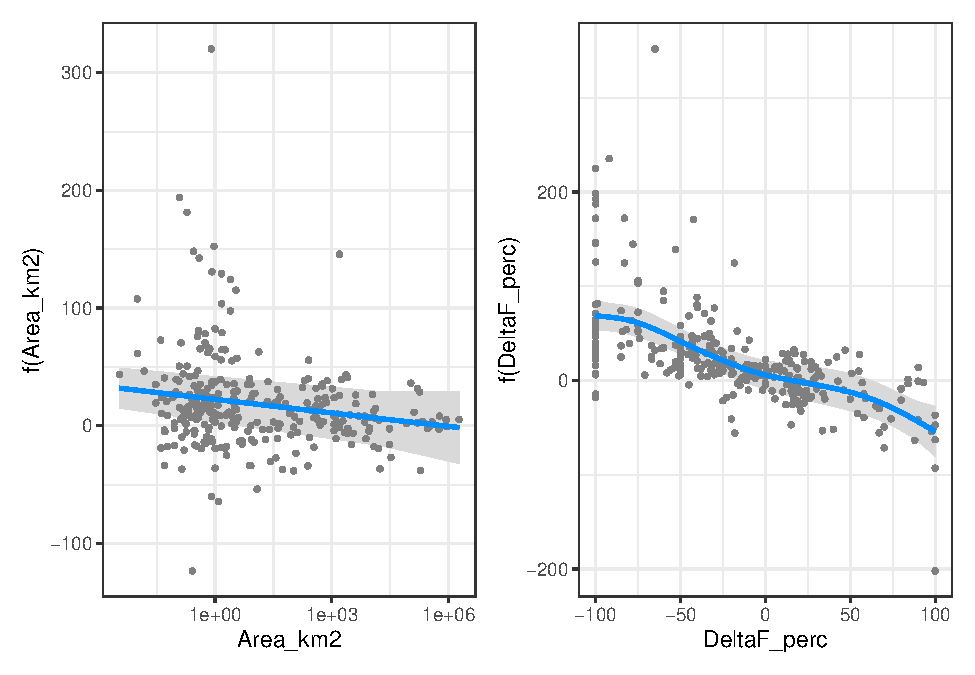
\includegraphics{SupplementaryMaterialPart3_files/figure-latex/unnamed-chunk-10-1.pdf}
The procedure \texttt{gam.check} highlights that the p-value of the Basis dimension check of the smooth on \texttt{DeltaF\_perc} is very small and the actual edf is close to 1 suggesting a linear relationship, similar to the smooth on log10(\texttt{Area\_km2}).

The residual analysis shows that including this non-linearity makes no difference in terms of he distribution of the residuals. While there is some remaining weak trend in the data, the overall distribution of the residuals is approximately normal.

\begin{Shaded}
\begin{Highlighting}[]
\FunctionTok{par}\NormalTok{(}\AttributeTok{mfrow=} \FunctionTok{c}\NormalTok{(}\DecValTok{2}\NormalTok{,}\DecValTok{2}\NormalTok{))}
\FunctionTok{gam.check}\NormalTok{(Forest\_model\_nonlin)}
\end{Highlighting}
\end{Shaded}

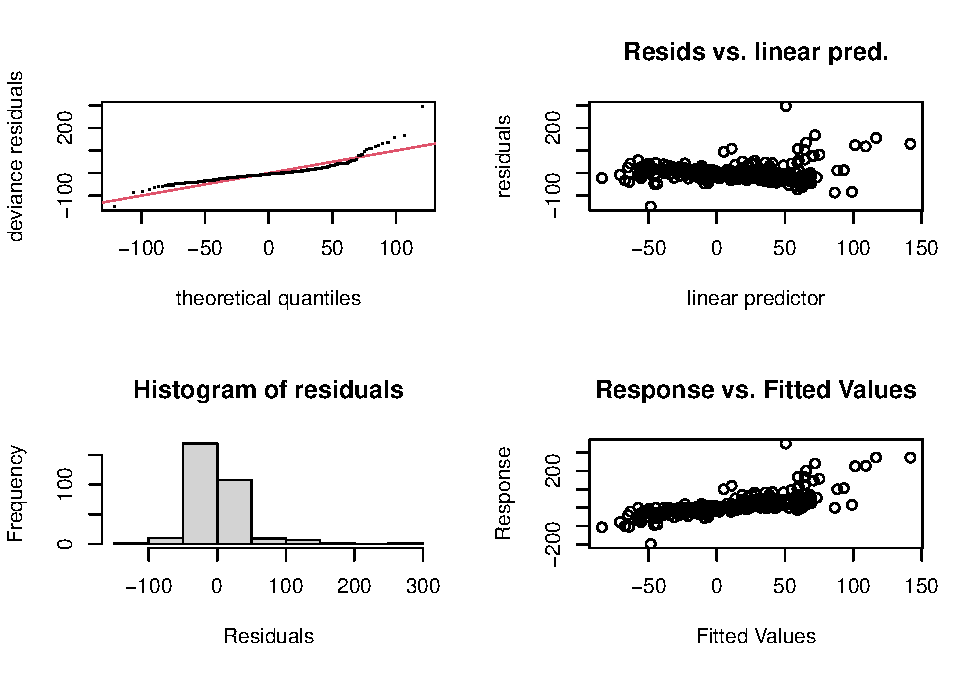
\includegraphics{SupplementaryMaterialPart3_files/figure-latex/unnamed-chunk-11-1.pdf}

\begin{verbatim}
## 
## Method: GCV   Optimizer: magic
## Smoothing parameter selection converged after 10 iterations.
## The RMS GCV score gradient at convergence was 0.005535096 .
## The Hessian was positive definite.
## Model rank =  69 / 69 
## 
## Basis dimension (k) checking results. Low p-value (k-index<1) may
## indicate that k is too low, especially if edf is close to k'.
## 
##                        k'    edf k-index p-value  
## s(DeltaF_perc)      9.000  4.476    0.91   0.080 .
## s(log10(Area_km2))  4.000  0.766    0.94   0.095 .
## s(Dryness)          9.000  4.698    0.94   0.100 .
## s(length)          34.000  4.645    0.94   0.090 .
## ---
## Signif. codes:  0 '***' 0.001 '**' 0.01 '*' 0.05 '.' 0.1 ' ' 1
\end{verbatim}

\renewcommand\refname{References}
\bibliography{forestandwater.bib}


\end{document}
